% sections/03_backgrounds_before_tagging.tex: generated by newdeck/html2beamer.py from the HTML deck, then edited by hand

% ---------------------------------------------------------------- slide 15: Outline
\begin{btframe}{}{Outline}
\begin{outlinelist}
\outlineitem{1}{Introduction}{the background types, the geometry, the input muons and neutrinos}{0.35}
\outlineitem{2}{Simulation}{transport, inelastic scattering, technologies, hits and digitisation, signal generation}{0.35}
\outlineitem{3}{Selection}{track cuts, pair cuts and time coincidence}{0.35}
\outlineitem{4}{Backgrounds before tagging}{μ and ν inelastic scattering, MS7 K\textsubscript{L}, combinatorial pairs}{1.00}
\outlineitem{5}{Background tagging}{rules, V0 rule, SBT model, R1, R2, summary}{0.35}
\outlineitem{6}{Optimisation and conclusion}{genetic-algorithm search, the optimised design Z1}{0.35}
\end{outlinelist}
\end{btframe}

% ---------------------------------------------------------------- slide 16: Muon inelastic scattering: in and around the vessel, and in MS7
\begin{btframe}{4 · Backgrounds before tagging · μ inelastic}{Muon inelastic scattering: in and around the vessel, and in MS7}
{\centering {\centering 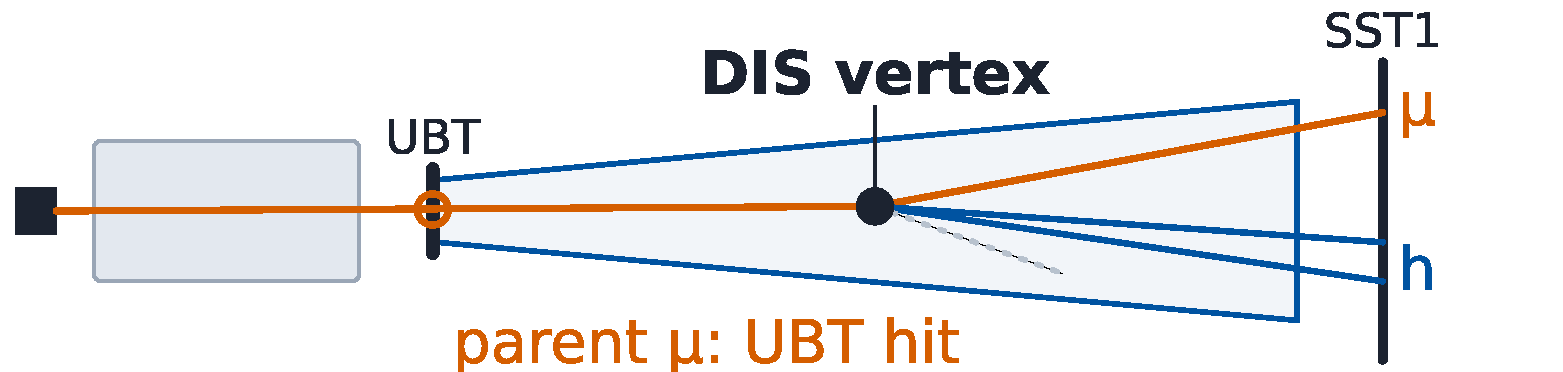
\includegraphics[width=1.00\linewidth,height=30pt,keepaspectratio]{figs/s15_sk1.pdf}\par}
\par}
\vspace{2.46pt}
{\fontsize{6.55pt}{6.92pt}\selectfont\setlength{\tabcolsep}{3.19pt}\renewcommand{\arraystretch}{1.42}
\begin{tabularx}{\linewidth}{>{\raggedright\arraybackslash}Xrrrrrr}
\textcolor{muted}{μ inelastic, per 15 years} & \textcolor{muted}{μ crossing (per spill)} & \textcolor{muted}{interactions} & \textcolor{muted}{≥ 2 good tracks} & \textcolor{muted}{pair cuts} & \textcolor{muted}{IP < 10 cm} & \textcolor{muted}{IP < 2.5 m} \\\headrule
helium & 8.4×10\textsuperscript{11} (5.6×10\textsuperscript{4}) & 1.3×10\textsuperscript{6} & (9.75 ± 0.04)×10\textsuperscript{4} & 8 830 ± 110 & 1 267 ± 40 & 8 740 ± 110 \\\rowrule
vessel walls & 8.4×10\textsuperscript{11} (5.6×10\textsuperscript{4}) & 2.2×10\textsuperscript{7} & (1.299 ± 0.005)×10\textsuperscript{6} & 1 680 ± 190 & 110 ± 49 & 1 460 ± 180 \\\rowrule
air around the vessel & 8.5×10\textsuperscript{11} (5.7×10\textsuperscript{4}) & 5.6×10\textsuperscript{6} & (2.29 ± 0.03)×10\textsuperscript{5} & 223 ± 79 & < 64 & 167 ± 68 \\\rowrule
air upstream of the vessel & 3.5×10\textsuperscript{11} (2.3×10\textsuperscript{4}) & 3.5×10\textsuperscript{5} & (1.381 ± 0.005)×10\textsuperscript{4} & 12.5 ± 1.5 & 1.2 ± 0.5 & 12.4 ± 1.5 \\\rowrule
UBT planes (material) & 5.8×10\textsuperscript{11} (3.9×10\textsuperscript{4}) & 3.1×10\textsuperscript{6} & (1.01 ± 0.01)×10\textsuperscript{5} & 2 030 ± 160 & 272 ± 59 & 2 030 ± 160 \\\rowrule
\end{tabularx}\par}
\vspace{2.46pt}
{\centering {\centering 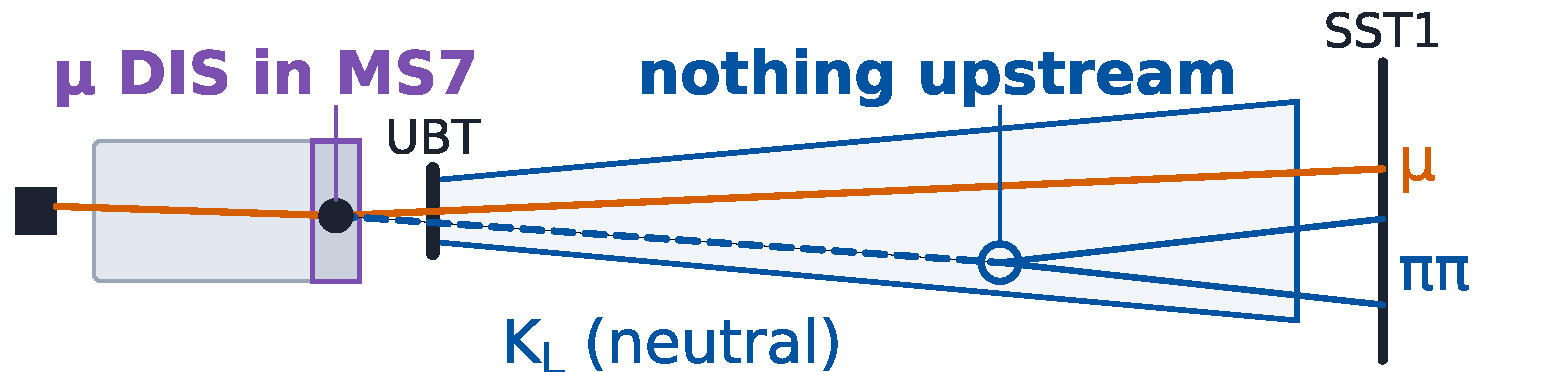
\includegraphics[width=1.00\linewidth,height=30pt,keepaspectratio]{figs/s15_sk2.pdf}\par}
\par}
\vspace{2.46pt}
{\fontsize{6.55pt}{6.92pt}\selectfont\setlength{\tabcolsep}{3.19pt}\renewcommand{\arraystretch}{1.42}
\begin{tabularx}{\linewidth}{>{\raggedright\arraybackslash}Xrrrrrr}
\textcolor{muted}{MS7 iron, last 50 cm, per 15 years} & \textcolor{muted}{μ crossing (per spill)} & \textcolor{muted}{interactions} & \textcolor{muted}{decays in vessel} & \textcolor{muted}{pair cuts} & \textcolor{muted}{IP < 10 cm} & \textcolor{muted}{IP < 2.5 m} \\\headrule
muons in the iron & 6.9×10\textsuperscript{15} (4.6×10\textsuperscript{8}) & 1.4×10\textsuperscript{13} & & & & \\\rowrule
K\textsubscript{L} & & & 3.0×10\textsuperscript{10} & 1.18×10\textsuperscript{7} & (1.27 ± 0.09)×10\textsuperscript{4} & (9.61 ± 0.05)×10\textsuperscript{6} \\\rowrule
K\textsuperscript{±} decaying in flight & & & 9.8×10\textsuperscript{10} & 2.3×10\textsuperscript{6} & (2.1 ± 0.9)×10\textsuperscript{3} & (1.86 ± 0.02)×10\textsuperscript{6} \\\rowrule
K\textsubscript{S}, Λ, Ξ\textsuperscript{0} & & & 1.3×10\textsuperscript{9} & 3 560 & 49 ± 49 & 3 560 \\\rowrule
\hline
\rowcolor{tint}\bfseries all & \bfseries  & \bfseries  & \bfseries  & \bfseries  & \bfseries (1.49 ± 0.13)×10\textsuperscript{4} & \bfseries (1.15 ± 0.01)×10\textsuperscript{7} \\\rowrule
\end{tabularx}\par}
\slidenote{MS7: P\textsubscript{int} = 2.0×10\textsuperscript{-3} per muon crossing the last 50 cm of iron (Kokoulin cross section, × 0.82 per nucleon in iron); “<”: no simulated event left, 90 \% CL upper limit 2.30 Σw\textsuperscript{2}/Σw.}
\begin{tikzpicture}[remember picture,overlay]
\node[anchor=north east,inner sep=0] (t1) at ([xshift=-14pt,yshift=-6pt]current page.north east) {
\includegraphics[width=125pt]{figs/talk_3.png}};
\node[anchor=north east,inner sep=0] at ([yshift=-2pt]t1.south east) {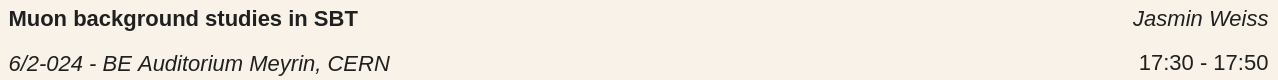
\includegraphics[width=125pt]{figs/talk_4.png}};
\end{tikzpicture}
\end{btframe}

% ---------------------------------------------------------------- slide 17: Neutrino inelastic scattering: helium, walls, tagger planes and MS7
\begin{btframe}{4 · Backgrounds before tagging · ν inelastic}{Neutrino inelastic scattering: helium, walls, tagger planes and MS7}
{\centering {\centering 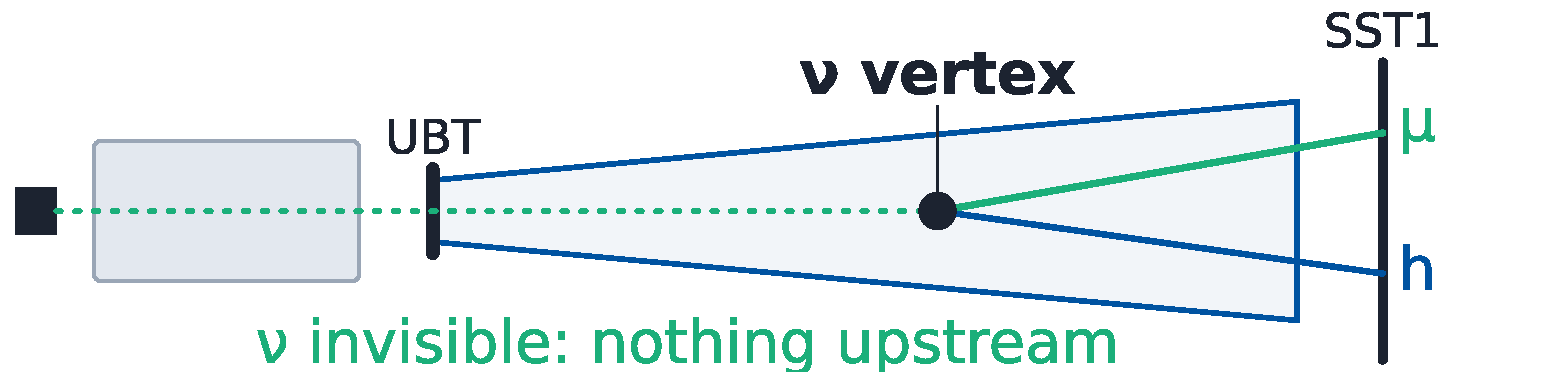
\includegraphics[width=1.00\linewidth,height=40.97pt,keepaspectratio]{figs/s16_sk1.pdf}\par}
\par}
\vspace{2.46pt}
{\fontsize{6.55pt}{7.83pt}\selectfont\setlength{\tabcolsep}{4.21pt}\renewcommand{\arraystretch}{1.42}
\begin{tabularx}{\linewidth}{>{\raggedright\arraybackslash}Xrrrrr}
\textcolor{muted}{ν inelastic, per 15 years} & \textcolor{muted}{interactions} & \textcolor{muted}{≥ 2 good tracks} & \textcolor{muted}{pair cuts} & \textcolor{muted}{IP < 10 cm} & \textcolor{muted}{IP < 2.5 m} \\\headrule
helium & 2.9×10\textsuperscript{4} & 3 231 ± 8 & 380 ± 2 & 3.1 ± 0.2 & 339 ± 2 \\\rowrule
vessel walls & 5.8×10\textsuperscript{4} & 1 581 ± 7 & 9.9 ± 0.5 & 0.02 ± 0.02 & 8.6 ± 0.4 \\\rowrule
air around & 5.0×10\textsuperscript{4} & 1 074 ± 7 & 0.6 ± 0.1 & < 0.04 & 0.5 ± 0.1 \\\rowrule
air upstream & 6518 & 176 ± 1 & 1.7 ± 0.1 & 0.04 ± 0.01 & 1.7 ± 0.1 \\\rowrule
UBT planes & 6.5×10\textsuperscript{4} & 1 287 ± 11 & 183 ± 4 & 2.7 ± 0.5 & 182 ± 4 \\\rowrule
MS7 iron & 2.0×10\textsuperscript{7} & (2.90 ± 0.04)×10\textsuperscript{5} & 820 ± 100 & 9.5 ± 6.5 & 800 ± 100 \\\rowrule
\hline
\rowcolor{tint}\bfseries total & \bfseries 2.0×10\textsuperscript{7} & \bfseries (2.98 ± 0.04)×10\textsuperscript{5} & \bfseries 1 400 & \bfseries 15 ± 7 & \bfseries 1 330 ± 100 \\\rowrule
\end{tabularx}\par}
\vspace{2.46pt}
{\centering {\centering 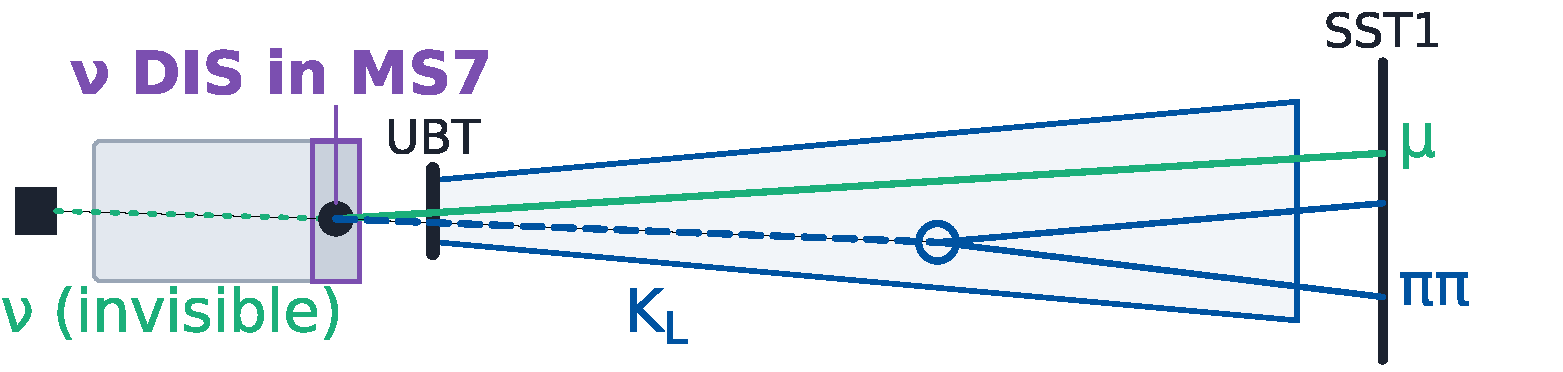
\includegraphics[width=1.00\linewidth,height=40.97pt,keepaspectratio]{figs/s16_sk2.pdf}\par}
\par}
\begin{tikzpicture}[remember picture,overlay]
\node[anchor=south west,inner sep=0] at ([xshift=14pt,yshift=26pt]current page.south west) {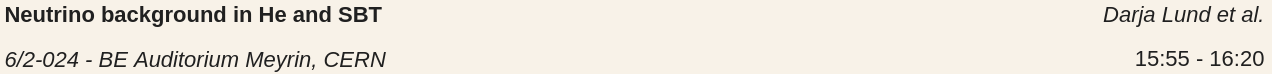
\includegraphics[width=140pt]{figs/talk_1.png}};
\end{tikzpicture}
\end{btframe}

% ---------------------------------------------------------------- slide 18: Combinatorial pairs: every cut, and all the pair types
\begin{btframe}{4 · Backgrounds before tagging · combinatorial}{Combinatorial pairs: every cut, and all the pair types}

{\centering 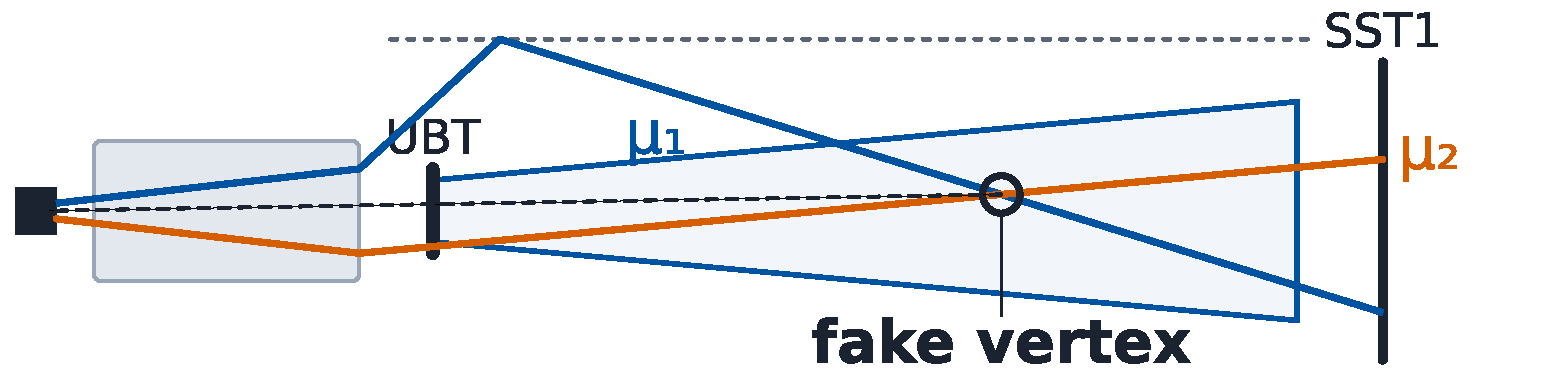
\includegraphics[width=1.00\linewidth,height=34.60pt,keepaspectratio]{figs/s17_sk1.pdf}\par}
\vspace{0.27pt}
{\centering \fontsize{6.01pt}{6.76pt}\selectfont μ × μ\par}
\par
\vspace{2.46pt}
{\fontsize{6.55pt}{7.83pt}\selectfont\setlength{\tabcolsep}{2.14pt}\renewcommand{\arraystretch}{1.42}
\begin{tabularx}{\linewidth}{l>{\raggedright\arraybackslash}Xrr}
\textcolor{muted}{cut} & \textcolor{muted}{} & \textcolor{muted}{per spill} & \textcolor{muted}{rejection} \\\headrule
track & in the SST1 acceptance & 3.19×10\textsuperscript{4} μ & – \\\rowrule
track & 4 straw stations + TD and p > 1 GeV (good tracks) & 6.3×10\textsuperscript{3} μ & ×5.0 \\\rowrule
pair & all pairs of good tracks in a spill & 2.1×10\textsuperscript{7} & – \\\rowrule
pair & opposite charge & 1.0×10\textsuperscript{7} & ×2.1 \\\rowrule
pair & DOCA < 1 cm & 1.9×10\textsuperscript{5} & ×54 \\\rowrule
pair & vertex 5 cm inside the vessel & 2 960 & ×63 \\\rowrule
pair & IP < 2.5 m (measured) & 2 310 & ×1.3 \\\rowrule
pair & IP < 10 cm (measured) & 121 & ×19 \\\rowrule
pair & time coincidence ±200 ps (× 4×10\textsuperscript{-10}) & 4.8×10\textsuperscript{-8} & ×2.5×10\textsuperscript{9} \\\rowrule
\rowcolor{tint}\bfseries 15 years & \bfseries × 1.5×10\textsuperscript{7} spills & \bfseries 0.73 (IP < 10 cm), 13.9 (IP < 2.5 m) & \bfseries  \\\rowrule
\end{tabularx}\par}
\vspace{2.46pt}

\end{btframe}

% ---------------------------------------------------------------- slide 19: combinatorial (2), restored 24 Nov 2026 with DOCA < 1 cm
\begin{btframe}{4 · Backgrounds before tagging · combinatorial (2)}{Combinatorial pairs: every cut, and all the pair types}
    
\begin{minipage}[t]{0.5\linewidth}
{\centering 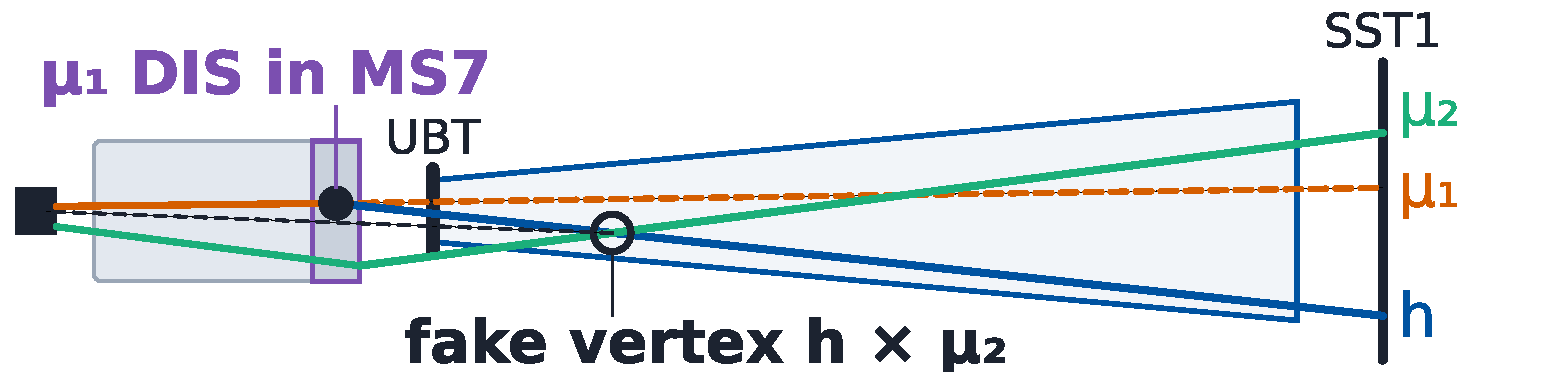
\includegraphics[width=1.00\linewidth,height=26pt,keepaspectratio]{figs/s17_sk2.pdf}\par}
\vspace{0.27pt}
{\centering \fontsize{6.01pt}{6.76pt}\selectfont μ × interaction product\par}
\end{minipage}%
\hfill%
\begin{minipage}[t]{0.5\linewidth}
{\centering 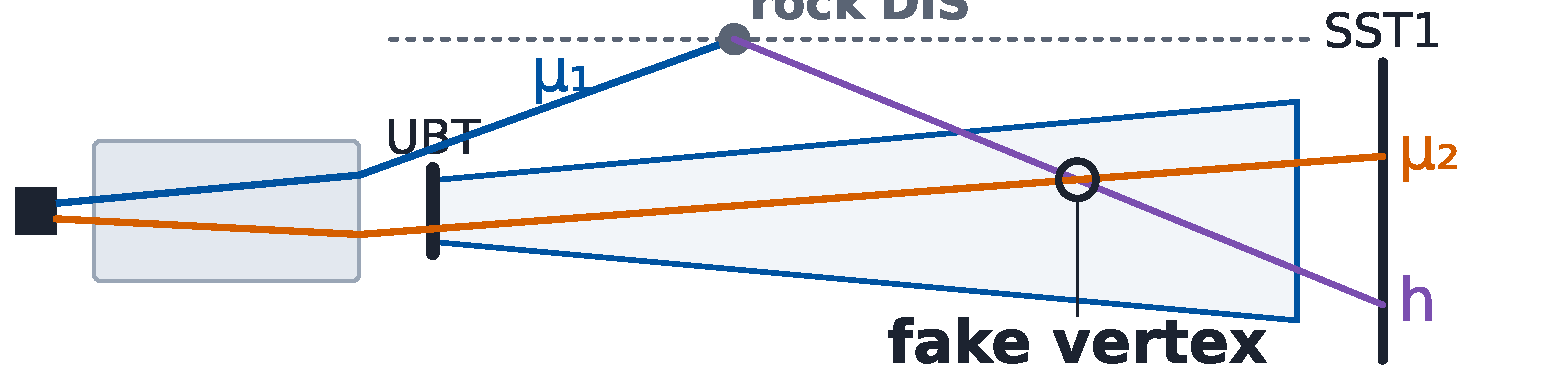
\includegraphics[width=1.00\linewidth,height=26pt,keepaspectratio]{figs/s17_sk3.pdf}\par}
\vspace{0.27pt}
{\centering \fontsize{5.01pt}{6.76pt}\selectfont μ × cavern-rock particle\par}
\end{minipage}
\vspace{2.46pt}
{\fontsize{6.2pt}{7.2pt}\selectfont\setlength{\tabcolsep}{2.14pt}\renewcommand{\arraystretch}{1.1}
\begin{tabularx}{\linewidth}{>{\raggedright\arraybackslash}Xrrr}
\textcolor{muted}{pairs per 15 years, ±200 ps, before tagging (DOCA < 1 cm; interactions with one track at SST1)} & \textcolor{muted}{pair cuts (no IP)} & \textcolor{muted}{IP < 10 cm} & \textcolor{muted}{IP < 2.5 m} \\\headrule
μ × μ & 14.3 & 0.73 & 13.9 \\\rowrule
\rowcolor{tint}\bfseries (MS7 μ interaction, 1 track) × μ & \bfseries 39.6 ± 1.4 & \bfseries 4.4 ± 0.3 & \bfseries 38.8 ± 1.4 \\\rowrule
(MS7 ν interaction, 1 track) × μ & 3.1×10\textsuperscript{-3} & 2.5×10\textsuperscript{-4} & 3.1×10\textsuperscript{-3} \\\rowrule
(vessel μ interaction, 1 track) × μ & 5.3×10\textsuperscript{-6} & 5×10\textsuperscript{-7} & 5.0×10\textsuperscript{-6} \\\rowrule
(vessel ν interaction, 1 track) × μ & 4.5×10\textsuperscript{-5} & 4.0×10\textsuperscript{-6} & 4.4×10\textsuperscript{-5} \\\rowrule
interaction × interaction (MS7 μ × MS7 μ) & 1.24 & 0.024 & 0.89 \\\rowrule
\rowcolor{tint}\bfseries (cavern-rock track) × μ &\bfseries  110 &\bfseries  42 &\bfseries  108 \\\rowrule
\rowcolor{tint}\bfseries total & \bfseries 165 & \bfseries 47 & \bfseries 162 \\\rowrule
\end{tabularx}\par}
\vspace{3pt}
{\centering 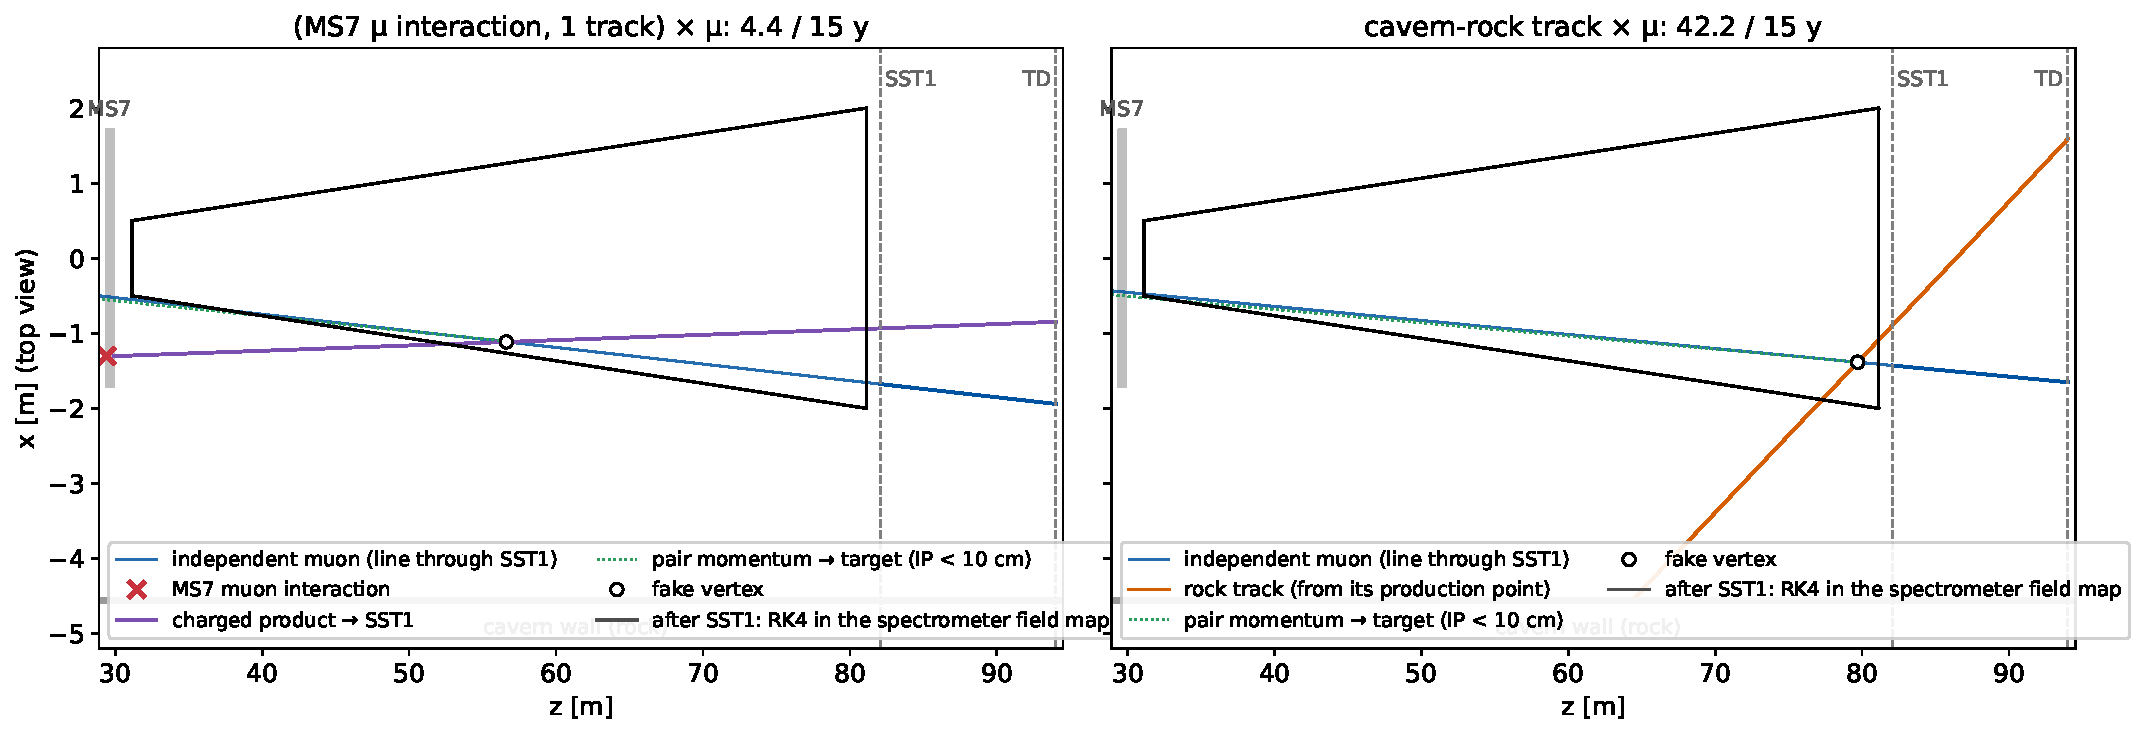
\includegraphics[width=0.92\linewidth,height=96pt,keepaspectratio]{figs/s20_pairs_tracks_doca1.pdf}\par}
\end{btframe}
